\documentclass[conference]{IEEEtran}
%\usepackage{cite}
\usepackage[backend=biber,citestyle=ieee]{biblatex}
\usepackage[T1]{fontenc}
\usepackage[utf8]{inputenc}
\usepackage{amsmath, amssymb, amsfonts}
\usepackage{algorithmic}
\usepackage{graphicx}
\usepackage{textcomp}
\usepackage{xcolor}
\usepackage{hyperref}
\usepackage{centernot}
\usepackage{caption}
\captionsetup[figure]{font=small}

\addbibresource{report.bib}

\graphicspath{{imgs}}
% What is this?
\def\BibTeX{{\rm B\kern-.05em{\sc i\kern-.025em b}\kern-.08em
    T\kern-.1667em\lower.7ex\hbox{E}\kern-.125emX}}


\begin{document}
\title{Data Science Final Project Report}
\author{\IEEEauthorblockN{Andr\'es Ponce}
		\IEEEauthorblockA{\textit{Department of Computer Science and Information Engineering} \\
		\textit{National Cheng Kung University} \\
		Tainan, Taiwan \\
		andresponce@ismp.csie.ncku.edu.tw}
}


\maketitle
\begin{abstract}
	Many e-commerce platforms need to search for similar or identical products
	given some query image.
	Doing so can increase the platform's ability to recommend interesting 
	products or analyze purchasing trends across product categories.
	For the eBay eProduct Visual Search Challenge, participants take a set
	of query images and search a large index set for images of matching products.
	We first train a model to recognize the hierarchical structure of the different
	image categories.
	Then, we use our model's output to produce hashes of the index images
	and query images using locality sensitive hashing, and locate identical products by comparing these hashes.
	This paper describes the motviation, approach, and results of the 
	comptetition.
\end{abstract}

\section{Introduction}
E-commerce platforms continue to grow and play a large role in consumer's
shopping behavior.
Especially with the pandemic, more people relied on such platforms for 
many of their purchases~\cite{jilkova2021digital}.

%PRODUCT PRODUCT PRODUCT %
Platforms where users directly sell their own products especially
benefit from finding images of identical products.
When a user searches for a product, he or she expects the results to contain
images of the same product.
On sites like eBay, identifying identical products can be very useful when 
aggregating sales of different listings of the same product.
Not only do e-commerce platforms rely on such visual search, but also visual
search engines such as Google Images, where the user can use an image as a query
instead of a search term.

The eBay eProduct Visual Recognition Challenge~\cite{jiangbo2021ebay} consists of
finding images of the same product from a large index set of images.
This challenge is one of fine-grained visual classification, since we are trying to 
find images of \emph{the same} product. 
Similar yet non-identical products can differ only by very fine details; likewise,
images of identical products can differ only in lighting conditions or other small
factors, increasing the difficulty of the task.
Despite the possibility for many small changes, our model should be resilient to such 
invariant factors and be able to distinguish similar products from each other.

\section{Competition Description}
\label{sec:description}
Current image datasets do not focus enough on super fine-grained object detection and classification.
This prompted the organizers to create the eProduct dataset focusing on fine-grained
visual recognition.
The dataset is divided into training, validation, and query sections. 

The training set consists of around 1.3 million labeled images modelled after the ImageNet~\cite{deng2009imagenet} dataset.
Each image comes with three levels of hierarchical labels: its meta class (16 total), level 2 class (17 total),
and the leaf class (1,000 total) as well as the product title and a unique identifier.
Also like ImageNet, the validation set contains 50,000 images, each containing the same information 
for each image as the training set.

The testing set contains 10,000 query images with only the unqiue identifier.
Given one of these query images, our task is to search for identical products to this query in a 1.1 million image index set, also provided
as part of the testing set.
The index set contains \emph{groundtruth sets} which are a match with any of the query images and 
a \emph{distractor set} which does not match with any query image.
Fig.~\ref{fig:structure} describes the structure of the dataset and the challenge posed by similar products.

\begin{figure}[!t]
\centering
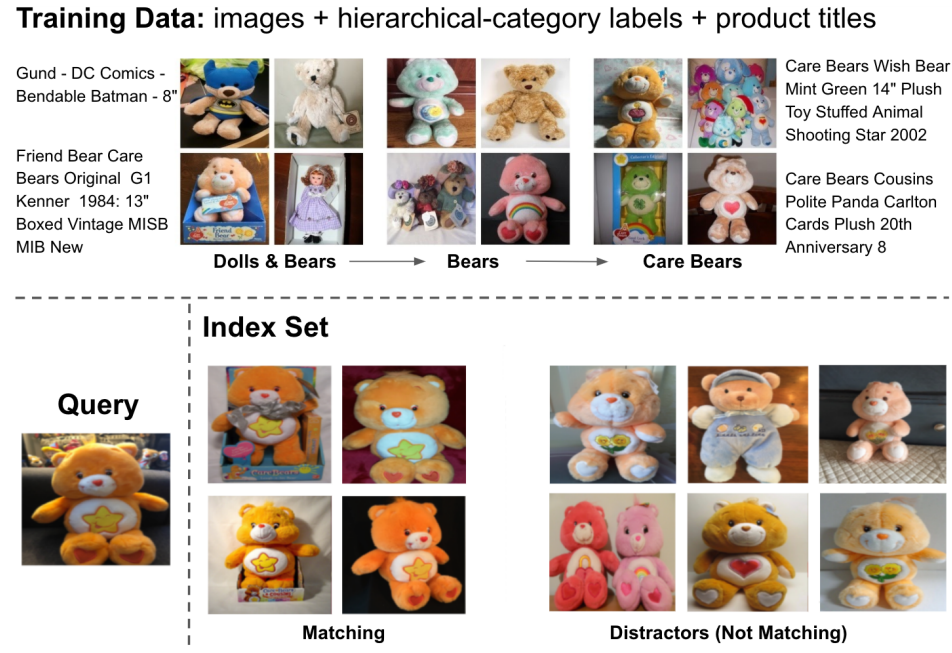
\includegraphics[scale=0.25]{structure}
\caption{eProduct dataset structure. The top section contains a sample training image and the meta,
level 2, and leaf categories. Each level contains a more specific type of product, and the leaf category
can still contain slightly different, non-matching products. 
The bottom section shows the query image and the identical products from the index set, along with a set 
of \emph{distractor} products that do not match with any query image.
Source:~\cite{jiangbo2021ebay}}

\label{fig:structure}
\end{figure}

\section{Related Work}
\label{sec:related}
There are many different approaches to dealing with image similarity and image 
ranking.
Listwise loss~\cite{revaud2019learning} tries to rank the images in an index set that are 
relevant to a particular query given binary labels of relevance. 
They split the interval $[-1, 1]$ into $M-1$ bins and calculate the average precision
of each bin for all the images in a batch.
Although this method addresses the same issue as the competition, it requires labels to know
if an image in the index set is relevant for a given query image.
During training, we only had access to the training set of images (not the query), and during 
evaluation the query images had no labels.
Thus it was unsuited for our competition.

Another approach~\cite{zhai2018classification} uses metric learning to better learn a discriminative 
function.
They obtain the weight $p_y$ of a class $y$ and maximize the product $x^T p_y$ over all classes.
This means that $p_y$ can act as a proxy for each class, and the greater the product with the feature
vector $x$ the greater the chance it belongs in that class.
By using the proxy information, the normalized softmax maximizes the distance between different class
proxies.
The class-balanced sampling benefits from larger batch sizes, which were not possible on our hardware.
Another issue for this approach is that the eProduct dataset is highly imabalanced, which means that 
if $S$ samples from $C$ classes were sampled each iteration, some inputs would be seen by our model
much more often than samples of other classes.
The datasets tested in the paper are not imbalanced.

Twin bottleneck hashing~\cite{shen2020auto} uses the output of a feature extractor $x\in\mathbb{R}^D$
to construct a continuous output $z$ and a binary hash vector $\boldsymbol{b}$.
The continuous $z$ passes through a Graph Convolutional Network (GNN) based on the adjacency
matrix $A$ built from the binary hashes in the batch.
The final result $z'$ goes through two fully connected layers that act as the decoder.
The proposed model seemed too complex for our problem, given it uses both a feature extractor and a GCN
trained in an adversarial way.

\section{Method Description}
The visual search problem can be divided into two major parts: training a deep model
to obtain an embedding $z$ and calculating the similarity between $z$ and the items in the index set.
We train a deep model for the first part and use locality sensitive hashing to find the 
similarities.

\begin{figure}[!t]
	\centering
	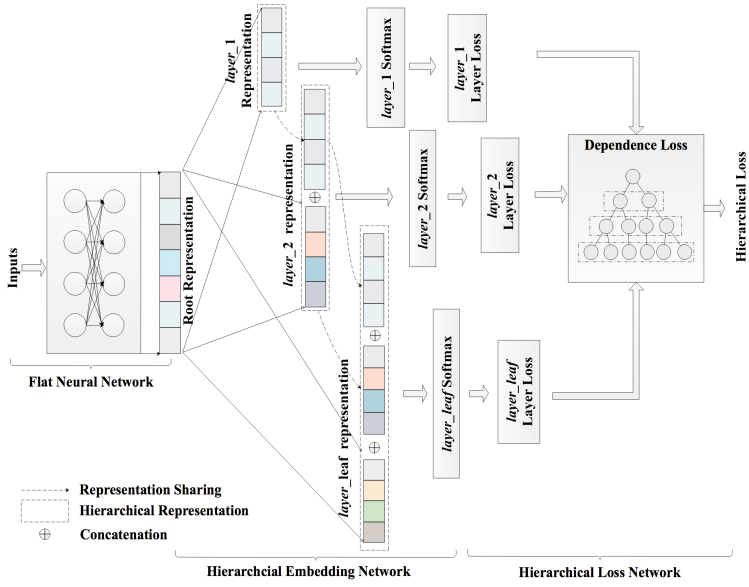
\includegraphics[scale=0.30]{network}
	\caption{Deep Hierarchical Embedding's structure . 
	The network first generates a representation for each hierarchical layer which is the concatenation
	of the prevoius layer's representation and the current layer. Then we calculate the loss
	function for each layer's prediction and use this to calculate dependence and hierarchical loss.
	Source:~\cite{gao2020deep}}
	\label{fig:network}
\end{figure}
\subsection{Deep Learning Model}
\label{sec:dlm}
The idea behind using a deep model is to obtain a vector $z$ that captures the important
information of an image.
The contents of the vector should be informed not only by the image contents, but also the 
hierarchical descriptions given as part of the training data.
Since there are three hierarchical levels of information (meta , level 2, and leaf),
our model should produce similar embeddings for products in similar categories.
This means our model should incorporate this information in some way during training.

However, the categories are not independent of each other.
For example, if a product belongs to a certain meta category, 
it can only belong to a subset of level 2 classes, and similar for 
leaf categories.
Our model should take these parent-child relationships into account.

We based our work on Deep Hierarchical Classification~\cite{gao2020deep} (DHC), since this model seemed 
specifically designed for hierarchical e-commerce classification.
The loss uses information from the hierarchies to make sure the child class and parent class actually
have this relationship.
With the meta, level 2, and leaf categories in our training data this method was appealing.

The architecture contains a flat neural network(FNN) $f(\theta)$ which generates a representation 
for each hierarchical layer $R'_l$. 
This representation is the concatenation of the previous hierarchical layer's representation
$R_l = R_{l-1}\oplus R'_l$ for $ l\neq 1$. 
The first layer's represnetation is not concatenated with anything else.
Each layer's representation passes through the softmax activation function.

The model contains two loss functions: the layer loss and dependence loss.
The layer loss for a hierarchical layer $l$ uses the output from the softmax 
function. 
\begin{equation}
		lloss_l = -\sum_{j=0}^{|l|} y_{lj} \log (\tilde{y}_{lj})
		\label{eq:lloss}
\end{equation}
where $y_{lj}$ is the expected output on the $j$th class of the $l$th hierarchical layer.

The dependence loss aims to capture the parent-child relationship among our predicted class labels
for hierarchical levels.
The loss function penalizes an incorrect parent-child relationship with terms $\mathbb{D}$ and $\mathbb{I}$.
The symbol $\mathbb{D}$ indicates whether our prediction for layer $l$ is a child of our prediction at layer $l-1$,
and $\mathbb{I}$ indicates whether our guess for the current layer is correct.
\begin{equation}
		dloss_l = -(ploss_{(l-1)})^{\mathbb{D}_{l}\mathbb{I}_{l-1}}(ploss_l)^{\mathbb{D}_l\mathbb{I}_l}
\end{equation}
where
\begin{equation*}
	\mathbb{D}_l = \left\{
			\begin{array}{ll}
					1~\textrm{if}~\hat{y}_l\centernot\implies \hat{y}_{(l-1)} \\ 
					0~\textrm{else}
			\end{array}
			\right.
			\label{eq:d}
\end{equation*}
\begin{equation*}
	\mathbb{I}_l = \left\{
			\begin{array}{ll}
				1~\textrm{if}~\hat{y}_l\neq y_l \\
				0~\textrm{else}
			\end{array}
			\right.
			\label{eq:i}
\end{equation*}

In our model, $ploss$ is set to a constant, and $\hat{y}\centernot\implies\hat{y}_{(l-1)}$ means
``$\hat{y}_l$ is \emph{not} the child of $\hat{y}_{(l-1)}$''.
Combining $lloss$ and $dloss$, we get our final loss function
\begin{equation}
		\mathcal{L}(\theta) = \sum_{i=1}^{L}\alpha_i lloss_i + \sum_{i=2}^{L}\beta_i dloss_{i}
		\label{eq:loss}
\end{equation}

Our task during training is to predict the three hierarchical classes of each image.

\subsection{Locality Sensitive Hashing}
Nearest-neighbor algorithms allow us to compare the similarity between two data items using some 
metric.
However, common algorithms would be prohibitive to run with millions of images in the index set.
Locality sensitive hashing(LSH)~\cite{rajaraman2011mining}~\cite{agrawal2019finding}~\cite{yona2018fast}~\cite{gupta2018locality}
finds \emph{approximate} nearest neighbors, sacrificing correctness for speed and scalability.
LSH hashes the inputs and assigns them to buckets, however LSH maximizes
the similarity of items in the same bucket.
Unlike regular hashing algorithms which try to minimize collisions, 
LSH tries to maximize the probability that items in the same bucket are of the 
same class.

Our hash function requires $k$ random hyperplanes that split some $d$-dimensional
space.
We then test whether the $i$th element in our point $a$ lies above or below the
$i$th hyperplane.
The string of ones and zeros becomes the item's hash.
Items close together in the embedding space will have similar hashes because they will
likely be above or below the hyperplanes in the same way.
The implementation of LSH is quite straightforward.
The hyperplanes are the columns of a randomly initialized matrix $W$.
The sign of the dot product $w_{j}^Ta$ tells us whether $a$ lies above
or below the $j$th hyperplane, and whether the $j$th character in the hash
string should be one or zero.

To query this hashtable, we hash the query item and retreive
all the items from the matching bucket.
We can use some metric such as cosine distance or hamming distance
to find the closest items in the bucket.

\section{Training and Experiments}
\label{sec:training}
We train a ResNet50~\cite{he2016deep} model to predict the classes at each 
hierarchical level for an input image.
That is, our model generates a prediction for the images meta class, level 2
class, and leaf class.
We use a learning rate of $0.0002$ and train for 12 epochs.
For data augmentations, we just resize the images to $64\times64$ and 
normalize.
Our validation accuracy after training was $73.8\%$ for meta class,
$66.9\%$ for level 2 class, and $51.5\%$ for leaf class.

After training our model, we had to construct the hashtable for the 
embeddings of the index set images.
We run each image through our model to obtain predictions for the 
three hierarchical levels and insert it to the hashtable.
The hashtable takes the input vector and produces a hash string  of length 20.
Originally, we concatenated the predictions for meta, level 2, and leaf node
into a 3-dimensional vector to index into the hash table.
After submitting our predictions, we found our accuracy to be quite low, so we
instead used the predictions for meta and level 2 class and the entire leaf 
node vector for a combined $1002$-dimensional vector to index to our hash table.
We found that changing the dimensionality of the vector did not have a large
impact on our predictions.


One of the main problems when inserting the index set embeddings was the size of the hashtable.
Since a single hashtable could not fit into main memory at once, 
we had to create a separate hashtable for every $8,000$ images, or $1,000$ batches, and write 
it separately to disk.
In the end we had $137$ hashtables to query per image, increasing
the computation cost of inference significantly.


When obtaining matches for the evaluation set, we run each image from the query set through 
our model to obtain the class predictions for each hierarchical level.
Using this embedding, we go through all the hashtables on disk and check
the most similar item in that hashtable.
For each table, we load it into memory, and query for the closest images.
For two hash sequences $h_1$ and $h_2$ we can define their cosine distance.

\begin{equation}
	\textrm{dist}(h_1, h_2) = 1 - \frac{h_1 \cdot h_2}{\|h_1\|\|h_2\|}
	\label{eq:cosinesim}
\end{equation}
The lower the cosine distance, the closer the two images are in the hash space 
and thus more similar.
In our experiments, we included all the images with a cosine distance smaller than $0.1$.
Following is a discussion of our results.

The competition used the mean average recall at $k$ (MAR@$k$) to evaluate submissions.
\begin{equation}
	\textrm{MAR@}k = \frac{1}{N}\sum_{i=1}^{N}R_i
	\label{eq:mar@k}
\end{equation}

The recall $R_i$ is the proportion of true matches in the top-$k$ recommendations.
The competition set $k = 10$.
\begin{equation}
	R_i = \frac{r_i}{g_i}
	\label{eq:recall}
\end{equation}

Using the methods as described, our MAR@10 was quite low -- around $3\%$.
Next, we propose some reasons why our model performed so poorly in the 
competition. 
Since we can no longer submit results, verifying our intuitions is 
not possible.

\section{Results Analysis}
In this section we analyse some of the reasons we believe led to poor performance on the 
competition.
\begin{enumerate}
		\item{The dataset is highly imbalanced.}
		\item{DHC trained and tested the model on CIFAR-100~\cite{krizhevsky2009learning}, which
				contains many less classes. The authors use their own split of the dataset and predict
				only two hierarchical layers.
		}
		\item{Overestimating importance of hierarchical information.}
		\item{Too high of a distance cuttoff, leading to excess of candidates.}
\end{enumerate}
\begin{figure}[!t]
		\centering
		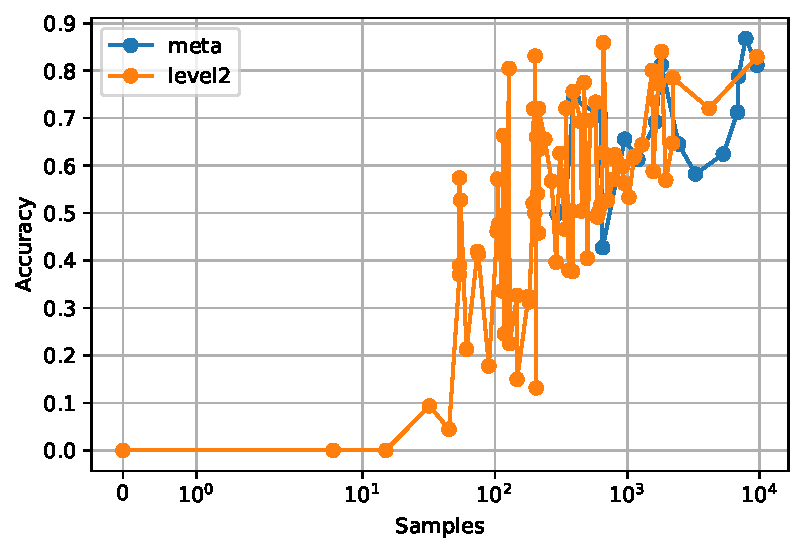
\includegraphics[scale=0.6]{accs}
		\caption{Sample number per class and accuracy in meta and level 2 categories
			on the validation set.
			Although less noticeable for meta class, there is a clear upward trend
			between sample number per class and model accuracy.
		}
		\label{fig:accs}
\end{figure}


\begin{figure}[!t]
		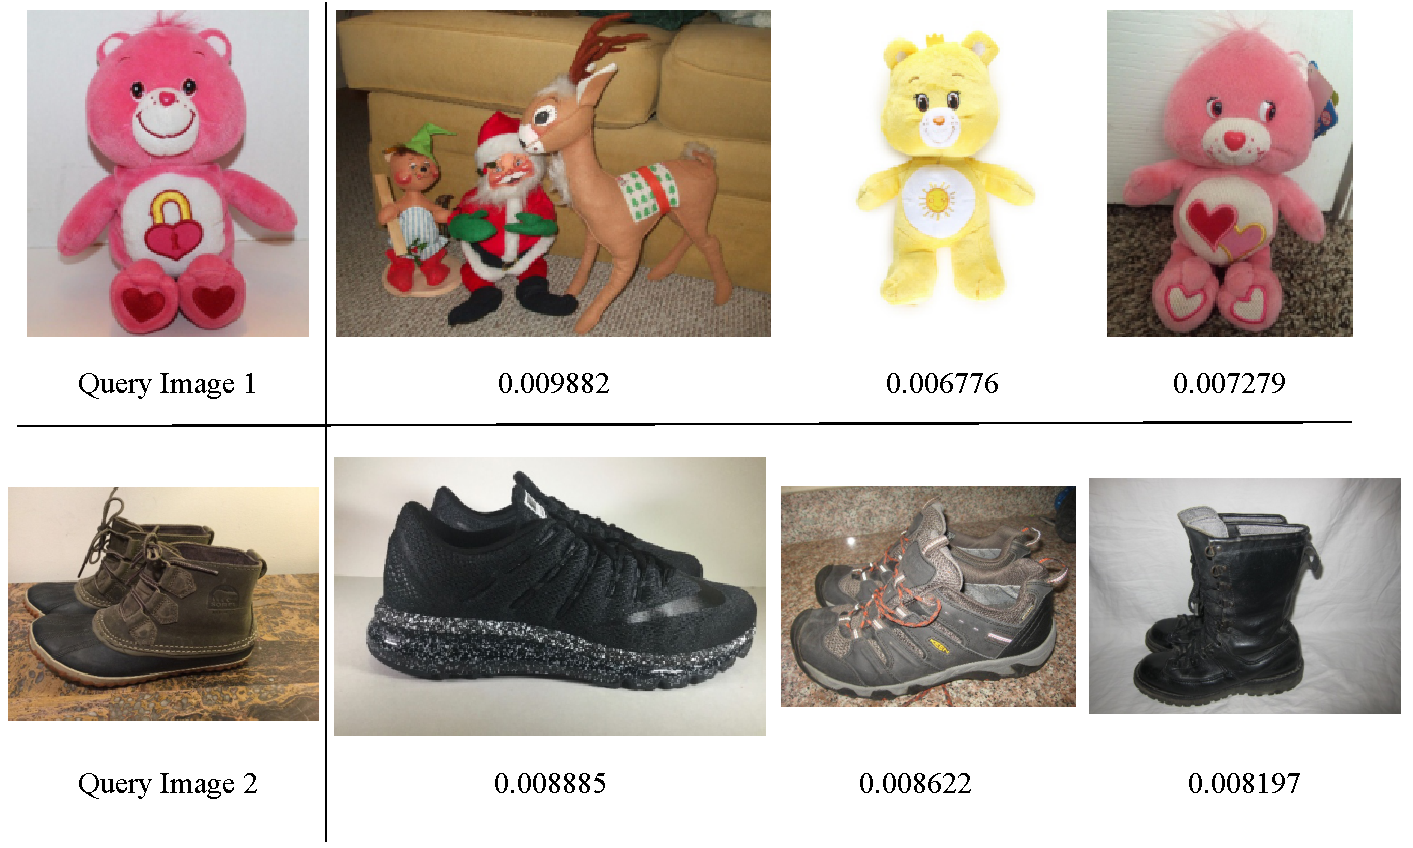
\includegraphics[width=0.5\textwidth]{retrieval}
		\caption{Sample query images and their cosine distances with some similar and dissimilar items in the matching set.
				Our model performs acceptably as a general image classifier, however it seems unable to learn fine-grained differences in the images.
				For instance, in the top row, most of the matching images are
		of other teddy bears, although sometimes our model can still misclassify quite different images as matching.
		In the bottom row, for a harder query, even images with the lowest distances are still quite different.
		This discrepancy between query images highlights the difficulty in setting a uniform distance cutoff.
		}
		\label{fig:retrieval}
\end{figure}

\subsection{Imbalanced Dataset}
This dataset is highly imbalanced, making it harder for our model to learn classes which do not contain many 
samples.
For instance, some categories have no samples in the training set.
\figurename\ref{fig:accs} shows our model's accuracy on the validation set changes with the number of samples for the 
meta and level 2 categories.
For the level 2 cateogires, our accuracy is very low for images with few samples, and there is still a large variance
with classes that have around 100-500 samples.
The hardest classes to predict are those with fewer samples.


\subsection{Different Class Numbers}
The CIFAR-100 dataset contains only $100$ classes each containing $600$ images.
The authors of DHC split the dataset according to coarse and fine labels.
That means that there are many times less images than our dataset.
Furthermore, the authors do not perform image retrieval tests, only classification.

%\subsection{Individual Hashtable Queries}
%The second issue concerns the cost of loading and querying roughly one thousand hashtables
%for every query image.
%During evaluation, getting the matches for a single image could take roughly one minute, and for all the query images
%($3,000$ total) took around two days.
%This meant that I could not carry out many modifications by the time the competition deadline arrived.
%Most sources~\cite{agrawal2019finding}~\cite{gupta2018locality} do not mention the case when 
\subsection{Overestimation of Hierarchical Information Relevance}
The training dataset, which was all that we had at the beginning of the competition,
contains three levels of hierarchical labels as described in Sec.~\ref{sec:description}.
When choosing a model, we thought that these labels could allow us to more precisely match
identical products.
In the final result, the label informaiton played little part in the hashing and embedding process.
It might be the case that the model embeddings did not have sufficient intra-class variance, 
and that all inputs that belonged to the same set of hierarchical classes resulted in embeddings that were too 
similar.
We want embeddings that are similar for objects that belong to the same category but not
\emph{so} similar that cannot further distinguish between different products.

\subsection{Too Lenient Distance}
The ideal is to minimize the cosine distance in Eq.~\ref{eq:cosinesim} for 
hashes of identical products.
Two identical images will have distance of $0$.
For our experiments, we considered all images with similarity less than 
$0.1$ as matches.
We believe this was too large, as some of the testing images had too many matches,
most of which were similar but not the same product.
Having a stricter distance requirement might have helped our precision, although as 
mentioned above, re-evaluating the query set would have taken too much time.
Since most of our team's submissions were made in the last couple of days before the 
end of the competition, it was not possible to run different experiments.

Coming up with a strict distance cutoff is quite challenging.
Fig.\ref{fig:retrieval} illustrates this dilemma for two sample query images.
In the first row, the cosine distance is given between a sample query image and 
images our model predicts as referring to the same product.
We show three samples from the matching set.
For the teddy bear, occasionally an unrelated image will have very low cosine distance;
however, the vast majority of matches are of other teddy bears or toys.
But not the \emph{same} teddy bear.
The second query image of a pair of shoes is harder for our model.
Even the images in the matching set with low distance are quite different.
Setting a uniform distance cutoff for similarity is tricky: too low and we can miss 
out on actual matches whose images differ, but too high and many false positives are
included.

Our model works as a general image classifier. 
Even in the shoe query image, the matching images are still mostly other shoes.
We believe the issue with our model comes down to the \emph{fine-grained} aspect of the 
competition.
Given many distractors, our model can only pick up that they are the same type of object
but not different products.

\section{Alternatives}
With a little more understanding of why our network failed to learn the fine-grained
features necessary, we can introduce some alternative approaches that might perform
better.
Sec.~\ref{sec:related} introduces other approaches we considered for our project
proposal; here we discuss other alternatives that we investigated having 
finished the project.

A popular recent approach to unlabeled data is self-supervised learning, where our model can still make
classification predictions without needing labels.
Models such as SimCLR~\cite{chen2020simple} take an image $x$ and produce two \emph{views} $x^a$ and $x^+$ by applying
different augmentations to the image.
The view $x^a$ is the anchor view, and we want to find $x^+$ from all the images in the batch.
The loss function is usually some form of contrastive loss, where similar images are pulled closer together
and different images are pushed further in the embedding space. 
Self-supervised learning could have been very helpful in this project.
For example, if our belief is correct that the hierarhcical labels in the training 
set were not as useful as we thought, that would leave us with just the unlabeled images.


Other methods specifically focus on fine-grained visual recognition.
In \cite{zheng2019towards} the authors project the image features onto a hypersphere and
minimize the Euclidean distance between positive samples.
This requires labeled samples to train, and the labels present in the eProduct dataset
might not be discriminative enough.
\cite{wei2017selective} uses unsupervised learning to add the activations of all
the feature maps after a pooling layer.
The idea is that if an area is activated in many feature maps, the likelihood is
higher that it contains an object.
The unsupervised aspect might be helpful in finding the fine-grained differences
between similar products.

\section{Conclusion}
Joining the eBay eProduct Visual Search Challenge was quite an educational experience.
We did not have any knowledge of visual search before joining this competition, and even though 
our performance left much to be desired, we learned to appreciate the complexity and 
requirements of this task.
Visual search aids discovery of interesting products and facilitates data aggregation 
by many innovative platforms such as eBay.
With millions of users, these platforms see many entries for the same product.
Understanding similar products can aid these platforms improve their service and 
better undertand their users.

Visual search also brings its unique challenges.
The sheer quantity of products on these platforms requires specialized methods.
For example, traditional nearest-neighbors algorithms do not scale to the point
required by many platforms.
For our hardware, storing the hashes of all the index images proved too big,
but for a platform with access to better hardware, storing a dataset such as the 
one used for the competition could still prove manageable.

\printbibliography
\end{document}
